\noindent
\begin{tabular}{c}
\begin{minipage}[b]{0.5\textwidth}
 \begin{exerciseS}[Semicilindro. Risultante delle forze]
  Si consideri la copertura rigida di un campo da calcio avente sezione semicircolare di
  raggio $\bar{R}=50\ m$ rappresentata schematicamente in figura. Sulla struttura 
  soffia un vento uniforme ($\rho=1.225\,kg/m^3$, $P_\infty=101325\ Pa$) in direzione 
  orizzontale con velocit\`{a} $U_\infty=15\,km/h$. Assumendo di poter approssimare la corrente esterna 
  come stazionaria, bidimensionale e a potenziale, si richiede di determinare:
  \begin{itemize}
   \item[1.1)] la distribuzione della pressione esterna sulla sezione della struttura;
   \item[1.2)] la risultante per unit\`{a} di apertura delle forze agenti sulla struttura, 
               ipotizzando che la pressione interna $P_i$ sia pari a $P_\infty$.
  \end{itemize}
  \vspace{2mm}
($P(\theta) = P_\infty+\frac{1}{2}\rho U_\infty^2(1-4\sin^2\!\theta)$, $\bm{F} = 425.35\mathbf{\hat{\bm{y}}}\ N/m$)
  \end{exerciseS}
\end{minipage}
\hspace{3mm}
\begin{minipage}[b]{0.35\textwidth}
   \begin{center}
   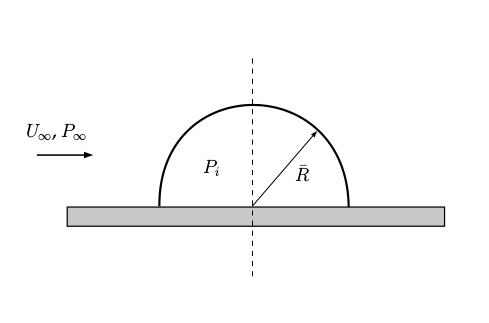
\includegraphics[width=1.50\textwidth]{./fig/Cyl.png}
   \end{center}
\end{minipage}
\end{tabular}


\sol

\partone
 Flusso non viscoso 2D, incomprimibile e irrotazionale attorno al cilindro. Circolazione.

\parttwo
 Una volta scritte (come si ricavano?) le componenti della velocità nel campo di moto, tramite il teorema di Bernoulli (nel caso incomprimibile, stazionario, inviscido, irrotazionale,...) si calcola la pressione agente sulla superficie del cilindro. Integrando gli sforzi di pressione (interna ed esterna al cilindro) sul contorno, si ottiene la risultante.

\begin{itemize}

\item Campo di moto nel dominio esterno alla metà cilindro ($(r,\theta) \in [0,\infty)\times[0,\pi])$.

\begin{equation}
\begin{cases}
  u_r (r,\theta) = U_\infty \displaystyle \left(1 - \frac{a^2}{r^2}\right)\cos{\theta} \\
  u_\theta (r,\theta) = - U_\infty \displaystyle \left(1 + \frac{a^2}{r^2}\right)\sin{\theta}
\end{cases}
\end{equation}

\item Grazie al teorema di Bernoulli (ipotesi...) si ottiene la pressione esterna sulla superficie della metà di cilindro. Sulla superficie del cilindro la componente radiale è nulla, quindi il modulo della velocità coincide con il valore assoluto della componente radiale.
\begin{equation}
\begin{aligned}
  P(\theta) & = P_\infty + \frac{1}{2}\rho U_\infty^2 - \frac{1}{2}\rho u_\theta(a,\theta)^2 = \\
            & = P_\infty + \frac{1}{2}\rho U_\infty^2 - \frac{1}{2}\rho (2 U_\infty \sin{\theta})^2 = \\
            & = P_\infty + \frac{1}{2}\rho U_\infty^2 (1 - 4 \sin^2{\theta})
\end{aligned}
\end{equation}

\item Integrale sulla superficie (interna ed esterna) degli sforzi di pressione per ottenere la risultante. Con $\hat{\bm{b}}$ si indica la normale diretta verso il centro del cilindro.

\begin{equation}
\begin{aligned}
  \bm{F} & = \int_{0}^{\pi} (P(\theta)-P_\infty) \hat{\bm{b}} a d\theta = \\
      & = \int_{0}^{\pi} (\frac{1}{2}\rho U_\infty^2 (1 - 4 \sin^2{\theta}) (-\cos{\theta}\hat{\bm{x}} - \sin{\theta}\hat{\bm{y}}) a d\theta = \\
\end{aligned}
\end{equation}

\vspace{0.2cm}
Usando i risultati (integrare!!)
\begin{equation}
\begin{aligned}
 & \int_{0}^{\pi} \sin{\theta} d\theta  = 2 \\
 & \int_{0}^{\pi} \cos{\theta} d\theta  = 0 \\
 & \int_{0}^{\pi} \sin^3{\theta} d\theta  = \frac{4}{3} \\
 & \int_{0}^{\pi} \cos{\theta}\sin^2{\theta} d\theta  = 0 
\end{aligned}
\end{equation}

si ottiene:
\begin{equation}
\begin{aligned}
  \bm{F} & = \int_{0}^{\pi} (P(\theta)-P_\infty) \hat{\bm{b}} a d\theta = \\
      & = - \frac{1}{2}\rho a U_\infty^2 \int_{0}^{\pi}  (1 - 4 \sin^2{\theta}) \sin{\theta}\hat{\bm{y}} d\theta = \\
      & = - \frac{1}{2}\rho a U_\infty^2 \displaystyle\left( 2 - \frac{16}{3}\right)\hat{\bm{y}} \\ \\
  \bm{F} & = \frac{5}{3}\rho a U_\infty^2 \hat{\bm{y}} \quad \Rightarrow \quad \bm{F} = 425.35 \hat{\bm{y}} N/m
\end{aligned}
\end{equation}


\end{itemize}
